\section{Conclusion}
\label{sec:conclusion}
We implemented a complete video-to-motion synthesis pipeline by deploying ViMo's transformer-diffusion architecture with two critical training enhancements: Min-SNR weighting and vectorized timestep sampling. Min-SNR dynamically reweights the diffusion loss to stabilize training across noisy timesteps, while vectorized sampling accelerates batch processing without sacrificing gradient fidelity. Together, these modifications eliminate the convergence fragility that typically plagues diffusion-based motion generation from casual video inputs.

The three-stage framework—vision acquisition, physics imitation, and adaptive policy refinement—processes unconstrained footage into simulation-ready control policies. Online adaptation compensates for kinematic errors and simulation mismatches during deployment, which proves essential when camera trajectories and editing styles vary unpredictably. Performance remains consistent across diverse capture conditions, confirming robustness beyond controlled datasets.

Current capabilities handle single-character motions reliably. Multi-person interactions and scene-level semantic constraints require extending the architecture to disentangle overlapping subjects and incorporate environment geometry. These directions build directly on the established foundation.

This implementation provides a practical baseline for generating physically plausible character motions directly from video, enabling applications in domains where traditional motion capture remains impractical.

%%%%%%%%%%%%%%%%%%%%%%%%%%%%%%%%%%%%%%%%%%%%%%%%%%%%%%%%%%%%%%%%%%%%%
\newpage
\section{Results}
\label{sec:results}

Two transformer–diffusion configurations are evaluated:
small model (\(d_{\text{model}} = 128\), \(n_{\text{heads}} = 4\)) and
big model (\(d_{\text{model}} = 256\), \(n_{\text{heads}} = 8\)).
For each setting, results include ground-truth reference frames,
deterministic predictions \(\hat{\mathbf{x}}_0\) at selected timesteps,
and stochastic samples drawn with the same conditioning.

\paragraph{\textbf{Small model v1, no PTSS (ViMo baseline), 50 epochs}}

\begin{figure}[H]
    \centering
    
\includegraphics[width=\textwidth]{outputs/d128_h4/run_v1_warm50/ground_truth_frames.png}
    \caption{Ground-truth motion sequence (small model v1, no PTSS).}
    \label{fig:run_v1_warm50_ground_truth_frames}
\end{figure}

\begin{figure}[H]
    \centering
    
\includegraphics[width=\textwidth]{outputs/d128_h4/run_v1_warm50/predicted_estimate_frames.png}
    \caption{Deterministic predictions \(\hat{\mathbf{x}}_0\) at timesteps
    \(t \in \{100, 200, 300, 400, 500\}\) (small model v1, no PTSS).}
    \label{fig:run_v1_warm50_predicted_estimates}
\end{figure}

\begin{figure}[H]
    \centering
\includegraphics[width=\textwidth]{outputs/d128_h4/run_v1_warm50/stochastic_generation_frames.png}
    \caption{Stochastic samples at timesteps
    \(t \in \{100, 200, 300, 400, 500\}\) (small model v1, no PTSS).}
    \label{fig:run_v1_warm50_stochastic_generations}
\end{figure}

%%%%%%%%%%%%%%%%%%%%%%%%%%%%%%%%%%%%%%%%%%%%%%%%%%%%%%%%%%%%%%%%%%%%%

\paragraph{\textbf{Small model v1 with PTSS, 65 epochs}}

\begin{figure}[H]
    \centering
    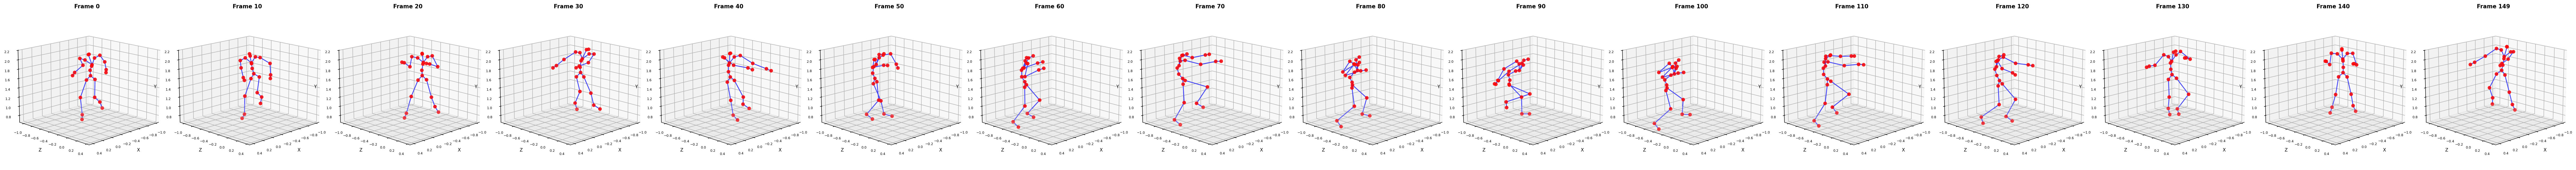
\includegraphics[width=\textwidth]{outputs/d128_h4/run_v1(sq)_ptss/ground_truth_frames.png}
    \caption{Ground-truth motion sequence (small model v1, PTSS).}
    \label{fig:run_v1sq_PTSS_ground_truth_frames}
\end{figure}

\begin{figure}[H]
    \centering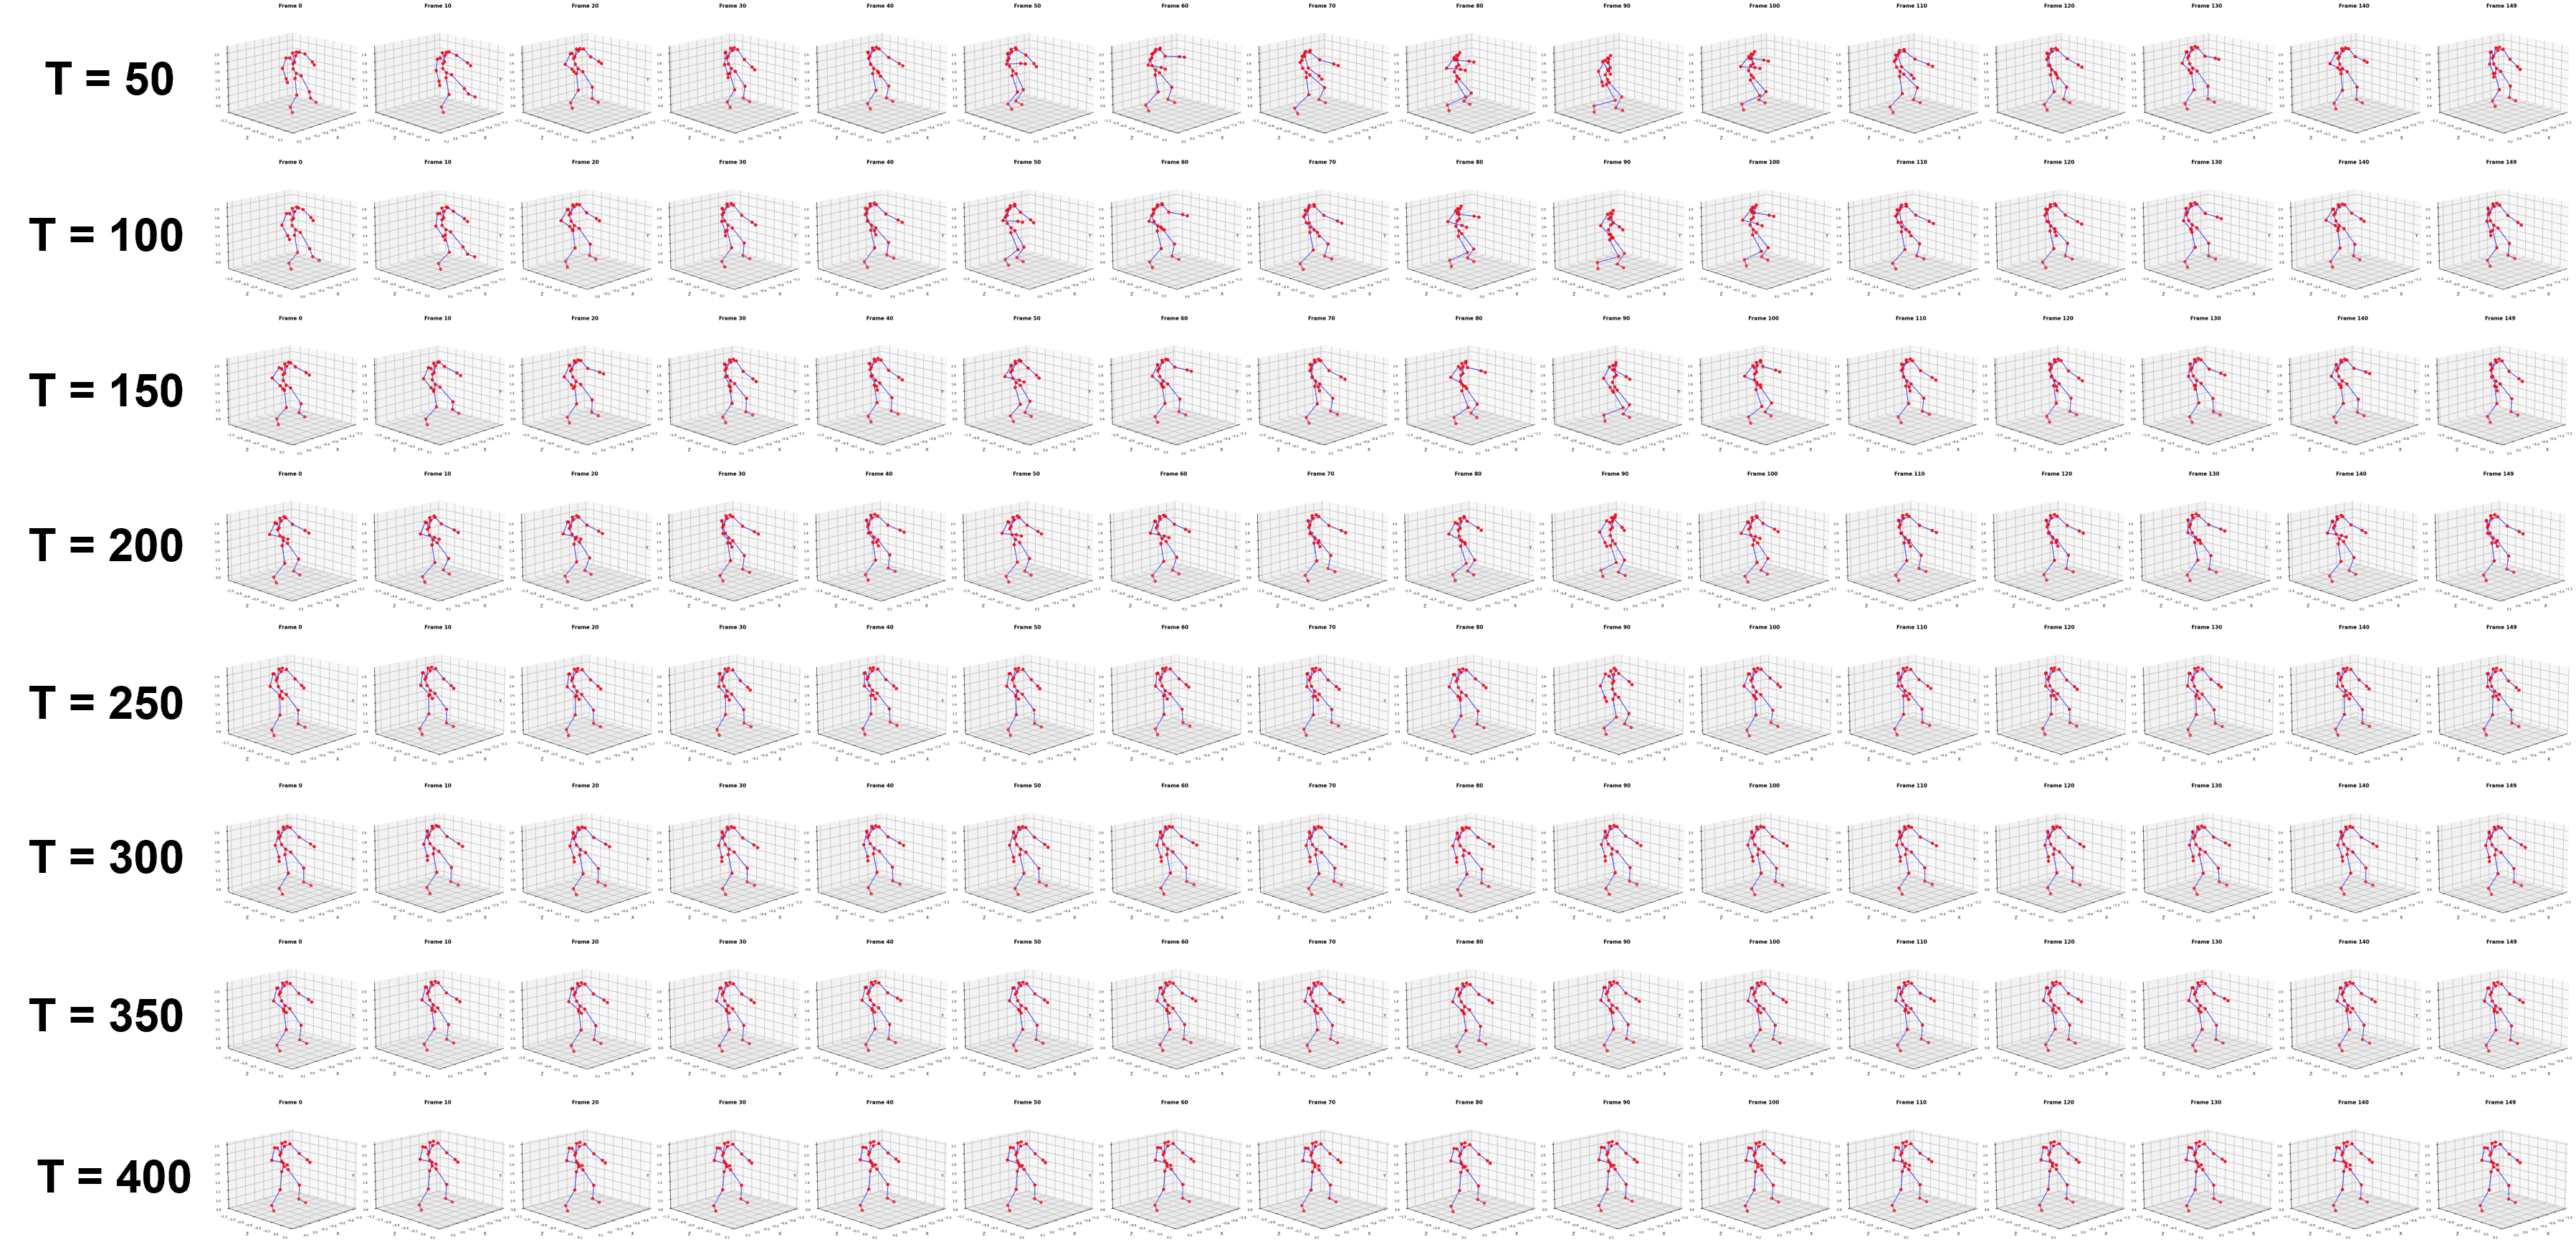
\includegraphics[width=\textwidth]{outputs/d128_h4/run_v1(sq)_ptss/predicted_estimate_frames.png}
    \caption{Deterministic predictions \(\hat{\mathbf{x}}_0\) at
    \(t \in \{50, 100, 150, 200, 250, 300, 350, 400\}\) (small model v1, PTSS).}
    \label{fig:run_v1sq_PTSS_predicted_estimates}
\end{figure}

\begin{figure}[H]
    \centering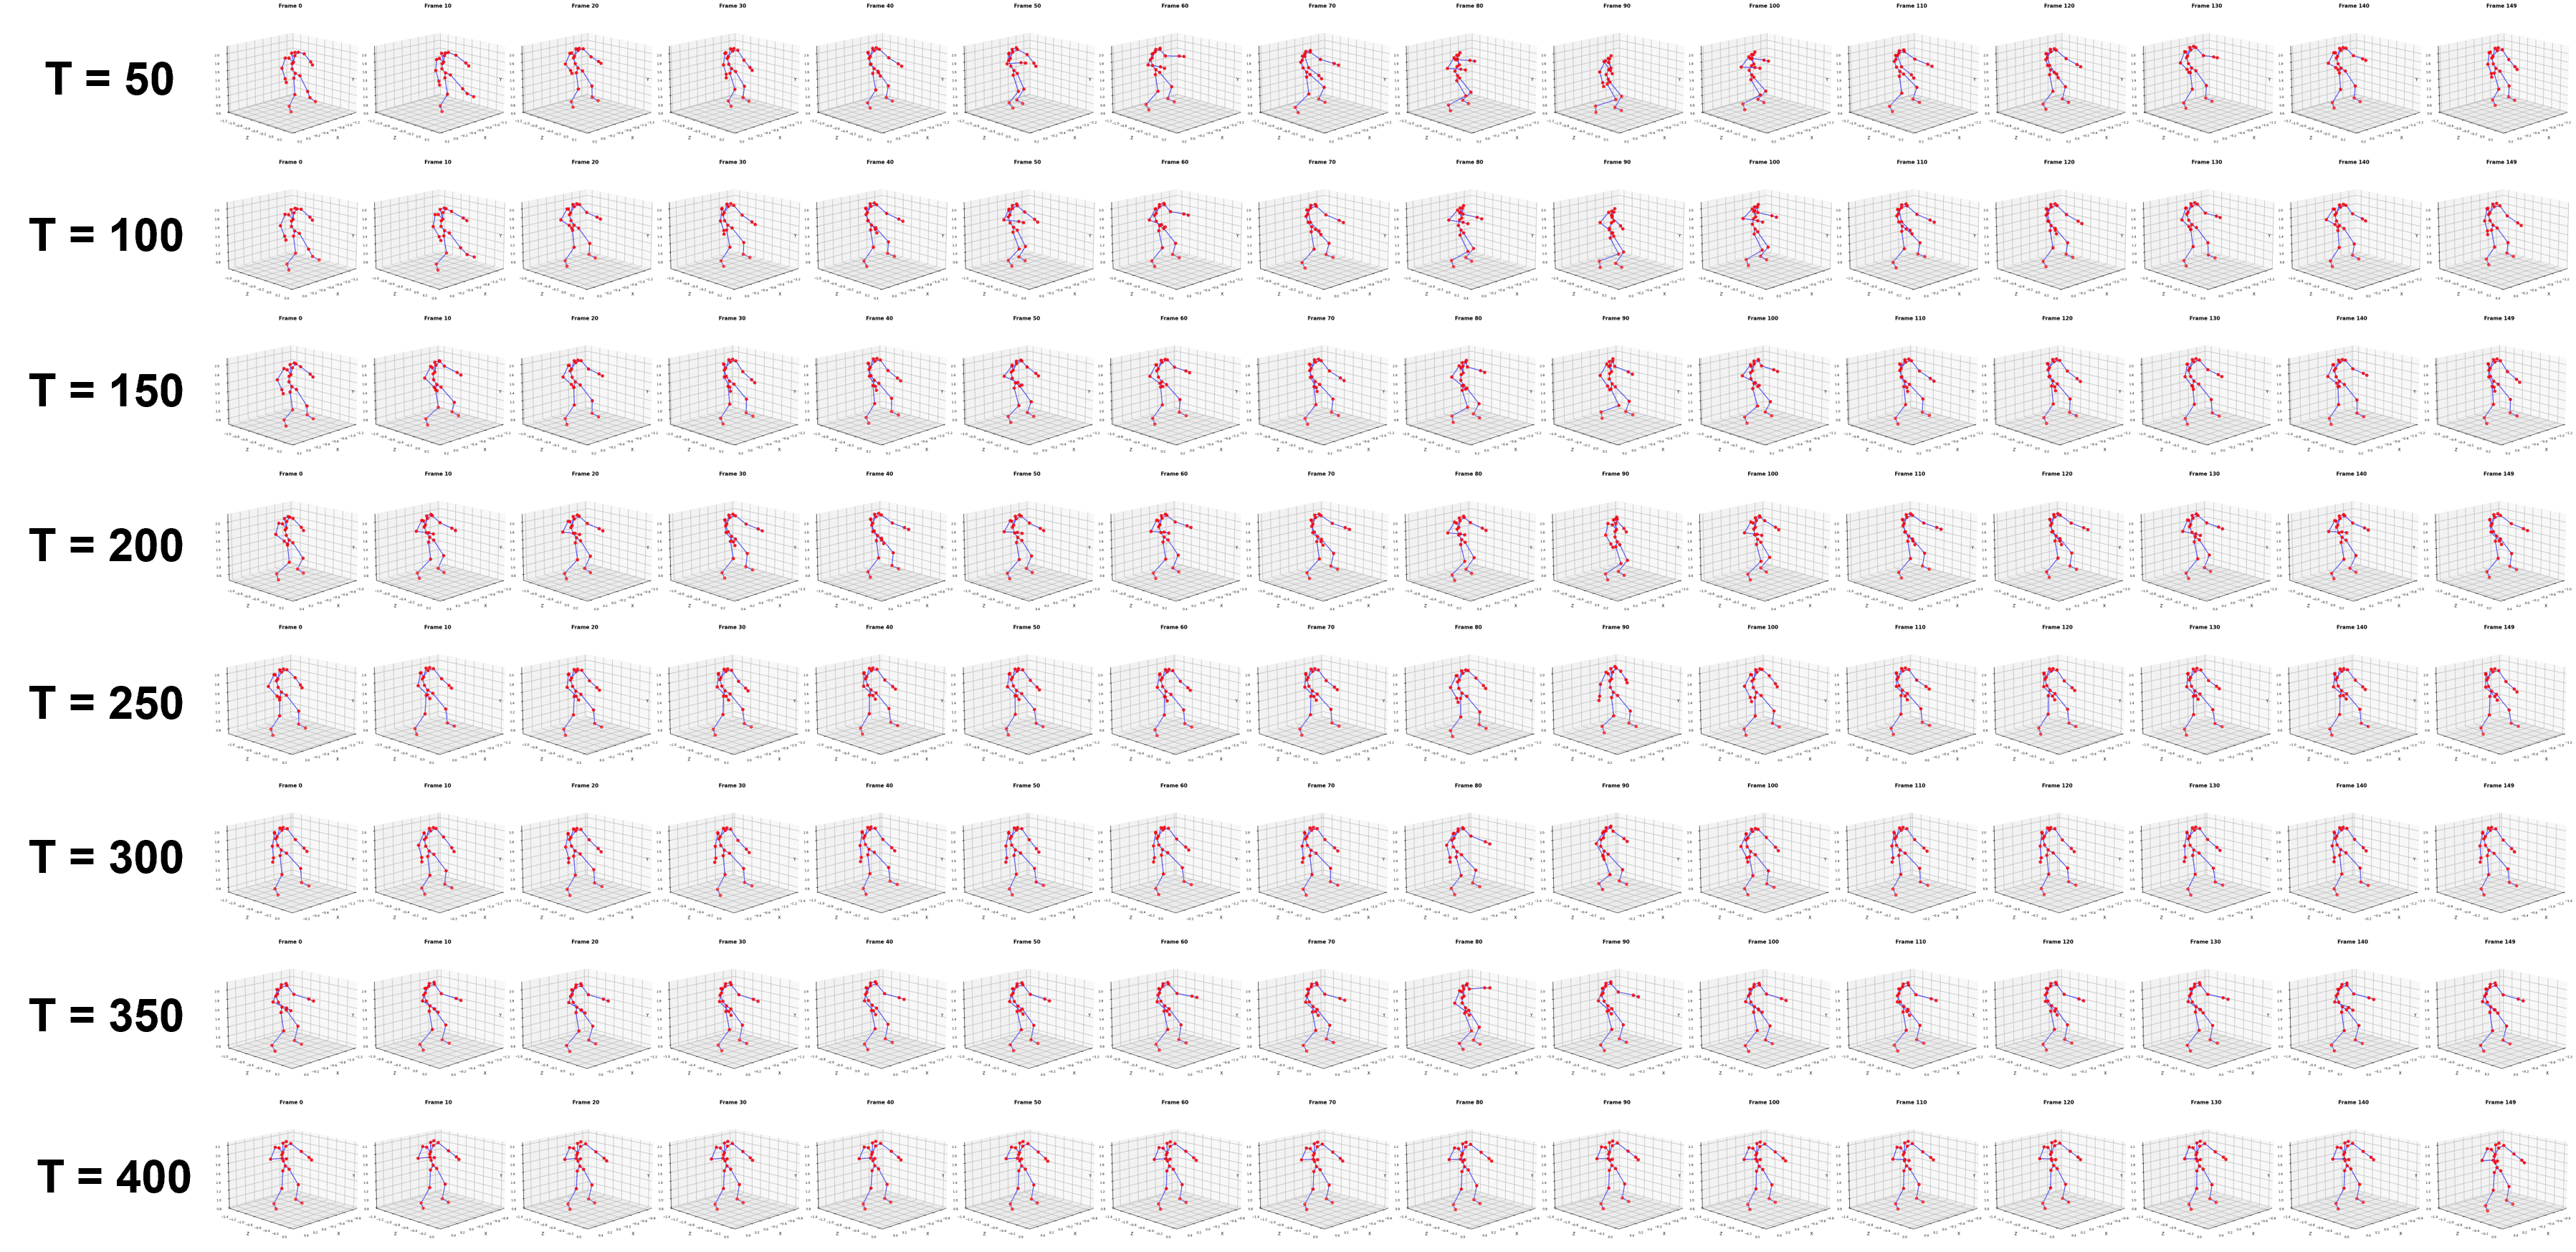
\includegraphics[width=\textwidth]{outputs/d128_h4/run_v1(sq)_ptss/stochastic_generation_frames.png}
    \caption{Stochastic samples at
    \(t \in \{50, 100, 150, 200, 250, 300, 350, 400\}\) (small model v1, PTSS).}
    \label{fig:run_v1sq_PTSS_stochastic_generations}
\end{figure}

%%%%%%%%%%%%%%%%%%%%%%%%%%%%%%%%%%%%%%%%%%%%%%%%%%%%%%%%%%%%%%%%%%%%%

\paragraph{\textbf{Small model v2 with PTSS, 65 epochs}}

\begin{figure}[H]
    \centering
\includegraphics[width=\textwidth]{outputs/d128_h4/run_v2(sq)_ptss/ground_truth_frames.png}
    \caption{Ground-truth motion sequence (small model v2, PTSS).}
    \label{fig:run_v2sq_PTSS_ground_truth_frames}
\end{figure}

\begin{figure}[H]
    \centering
\includegraphics[width=\textwidth]{outputs/d128_h4/run_v2(sq)_ptss/predicted_estimate_frames.png}
    \caption{Deterministic predictions \(\hat{\mathbf{x}}_0\) at
    \(t \in \{50, 100, 150, 200, 250\}\) (small model v2, PTSS).}
    \label{fig:run_v2sq_PTSS_predicted_estimates}
\end{figure}

\begin{figure}[H]
    \centering
\includegraphics[width=\textwidth]{outputs/d128_h4/run_v2(sq)_ptss/stochastic_generation_frames.png}
    \caption{Stochastic samples at
    \(t \in \{50, 100, 150, 200, 250\}\) (small model v2, PTSS).}
    \label{fig:run_v2sq_PTSS_stochastic_generations}
\end{figure}

%%%%%%%%%%%%%%%%%%%%%%%%%%%%%%%%%%%%%%%%%%%%%%%%%%%%%%%%%%%%%%%%%%%%%

\paragraph{\textbf{Big model v1 with PTSS, 100 epochs}}

\begin{figure}[H]
    \centering
    
\includegraphics[width=\textwidth]{outputs/d256_h8/run_v1(sq) PTSS/ex1/ground_truth_frames.png}
    \caption{Example 1: ground-truth motion sequence (big model v1, PTSS).}
    \label{fig:d256_h8_ex1_ground_truth_frames}
\end{figure}

\begin{figure}[H]
    \centering
    
\includegraphics[width=\textwidth]{outputs/d256_h8/run_v1(sq) PTSS/ex1/predicted_estimate_frames.png}
    \caption{Example 1: deterministic predictions \(\hat{\mathbf{x}}_0\) at
    \(t \in \{50, 100, 150, 200, 250, 300, 350, 400, 450\}\) (big model v1, PTSS).}
    \label{fig:d256_h8_ex1_predicted_estimates}
\end{figure}

\begin{figure}[H]
    \centering
    
\includegraphics[width=\textwidth]{outputs/d256_h8/run_v1(sq) PTSS/ex1/stochastic_generation_frames.png}
    \caption{Example 1: stochastic samples at
    \(t \in \{50, 100, 150, 200, 250, 300, 350, 400, 450\}\) (big model v1, PTSS).}
    \label{fig:d256_h8_ex1_stochastic_generations}
\end{figure}

\begin{figure}[H]
    \centering
    
\includegraphics[width=\textwidth]{outputs/d256_h8/run_v1(sq) PTSS/ex2/ground_truth_frames.png}
    \caption{Example 2: ground-truth motion sequence (big model v1, PTSS).}
    \label{fig:d256_h8_ex2_ground_truth_frames}
\end{figure}

\begin{figure}[H]
    \centering
    
\includegraphics[width=\textwidth]{outputs/d256_h8/run_v1(sq) PTSS/ex2/predicted_estimate_frames.png}
    \caption{Example 2: deterministic predictions \(\hat{\mathbf{x}}_0\) at
    \(t \in \{50, 100, 150, 200, 250, 300, 350\}\) (big model v1, PTSS).}
    \label{fig:d256_h8_ex2_predicted_estimates}
\end{figure}

\begin{figure}[H]
    \centering
    
\includegraphics[width=\textwidth]{outputs/d256_h8/run_v1(sq) PTSS/ex2/stochastic_generation_frames.png}
    \caption{Example 2: stochastic samples at
    \(t \in \{50, 100, 150, 200, 250, 300, 350\}\) (big model v1, PTSS).}
    \label{fig:d256_h8_ex2_stochastic_generations}
\end{figure}


